\subsubsection{Effect of Pileup on Dijet Balance}

The effect of the number of pileup vertices, NPV, and the mean number of interactions per bunch crossing, $\mu$, on the relative response from the matrix method are presented in this section.
Figure \ref{JetPerf:NPV_Mu} shows (a) the NPV distribution and (b) the $\mu$ distributions.
Three NPV regions are defined to select different pileup conditions, \Range{NPV}{0}{2}, \Range{NPV}{3}{6}, and  $\rm NPV\ge7$, with an average NPV of 2.48, 4.48 and 7.71 respectively. 
Two NPV regions are defined, \Range{\mu}{0}{7} and  $\mu > 7$, with an average $\mu$ of 5.33 and 9.94 respectively. 
Data points which have no cuts on $\mu$ or NPV are also shown, which have an average NPV and $\mu$ of 5.19 and 6.48.


%High NPV:  Ave NVP:  7.71314
%Med NPV:  Ave NVP:  4.48111
%Low NPV:  Ave NVP:  2.47613
%Standard: Average mu : 6.47532  Ave NVP:  5.18579


Figure \ref{JetPerf:PileupComp_j10} shows the relative response as a function of detector $\eta$ for jets with $22<\ptave{}<30$ GeV.
At low pileup there is generally a lower response outside of the reference region, whereas at higher pileup the response is close to unity. 
Figure \ref{JetPerf:PileupComp_j15} shows the relative response for jets with $30<\ptave{}<40$ GeV.
Again, in low pileup conditions the relative response is lower. 
However, in higher pileup conditions the relative response is higher in the forward regions.
Figure \ref{JetPerf:PileupComp_j20} shows the relative response for jets with $40<\ptave{}<55$ GeV.
The different pileup conditions result in very similar  relative responses, indicating that pileup has less effect at higher jet \pt{}.
The explaination is that pileup can be considered to contribute and average ammount of energy thoughout the detector.
For low \pt{} jets, this can significantly increase their \pt{}. 
However for higher \pt{} jets, this increase in energy is small compared to the total \pt{} of the jet. 

Figures \ref{JetPerf:MuComp_j10} - \ref{JetPerf:MuComp_j20} show the relative response as a function of detector $\eta$ for low, medium and high $\mu$ and the whole dataset. 
Within the statistical error bars, all the results show a less than 3 percent spread, even in the lowest \ptave{} bin.
***********Note here that the Low Mu has low stats, so I will ignore it in the explanation and remake the plots with just 2 curves on.  ******

The observed effects from NPV and $\mu$ are relatively small, and are covered by the uncertainty in the jet pileup correction, and therefore do not need to be added to the JES uncertainty from the dijet balance.
\begin{figure}
\centering
\mbox{
              \subfigure[]{\epsfig{figure=figures/JetPerformance/2011/NPVDist.eps,width=0.5\textwidth}}\quad
              \subfigure[]{\epsfig{figure=figures/JetPerformance/2011/MuDist.eps,width=0.5\textwidth}}\quad
                              }
\caption[]{
(a) The NPV distribution and (b) the $\mu$ distribution for 2011 data.
\label{JetPerf:NPV_Mu}}
\end{figure}



\begin{figure}
\centering
\mbox{
              \epsfig{figure=figures/JetPerformance/2011/ResponseNPVj10Comp.eps,width=0.9\textwidth}
}
\caption[]{
Relative response as a function of detector $\eta$ for jets with $22<\ptave{}<30$ GeV.
Relative responses are shown for events with \Range{NPV}{0}{2}, \Range{NPV}{3}{6}, $\rm NPV\ge7$ and all NPV. 
\label{JetPerf:PileupComp_j10}}
\end{figure}



\begin{figure}
\centering
\mbox{
              \epsfig{figure=figures/JetPerformance/2011/ResponseNPVj15Comp.eps,width=0.9\textwidth}
              %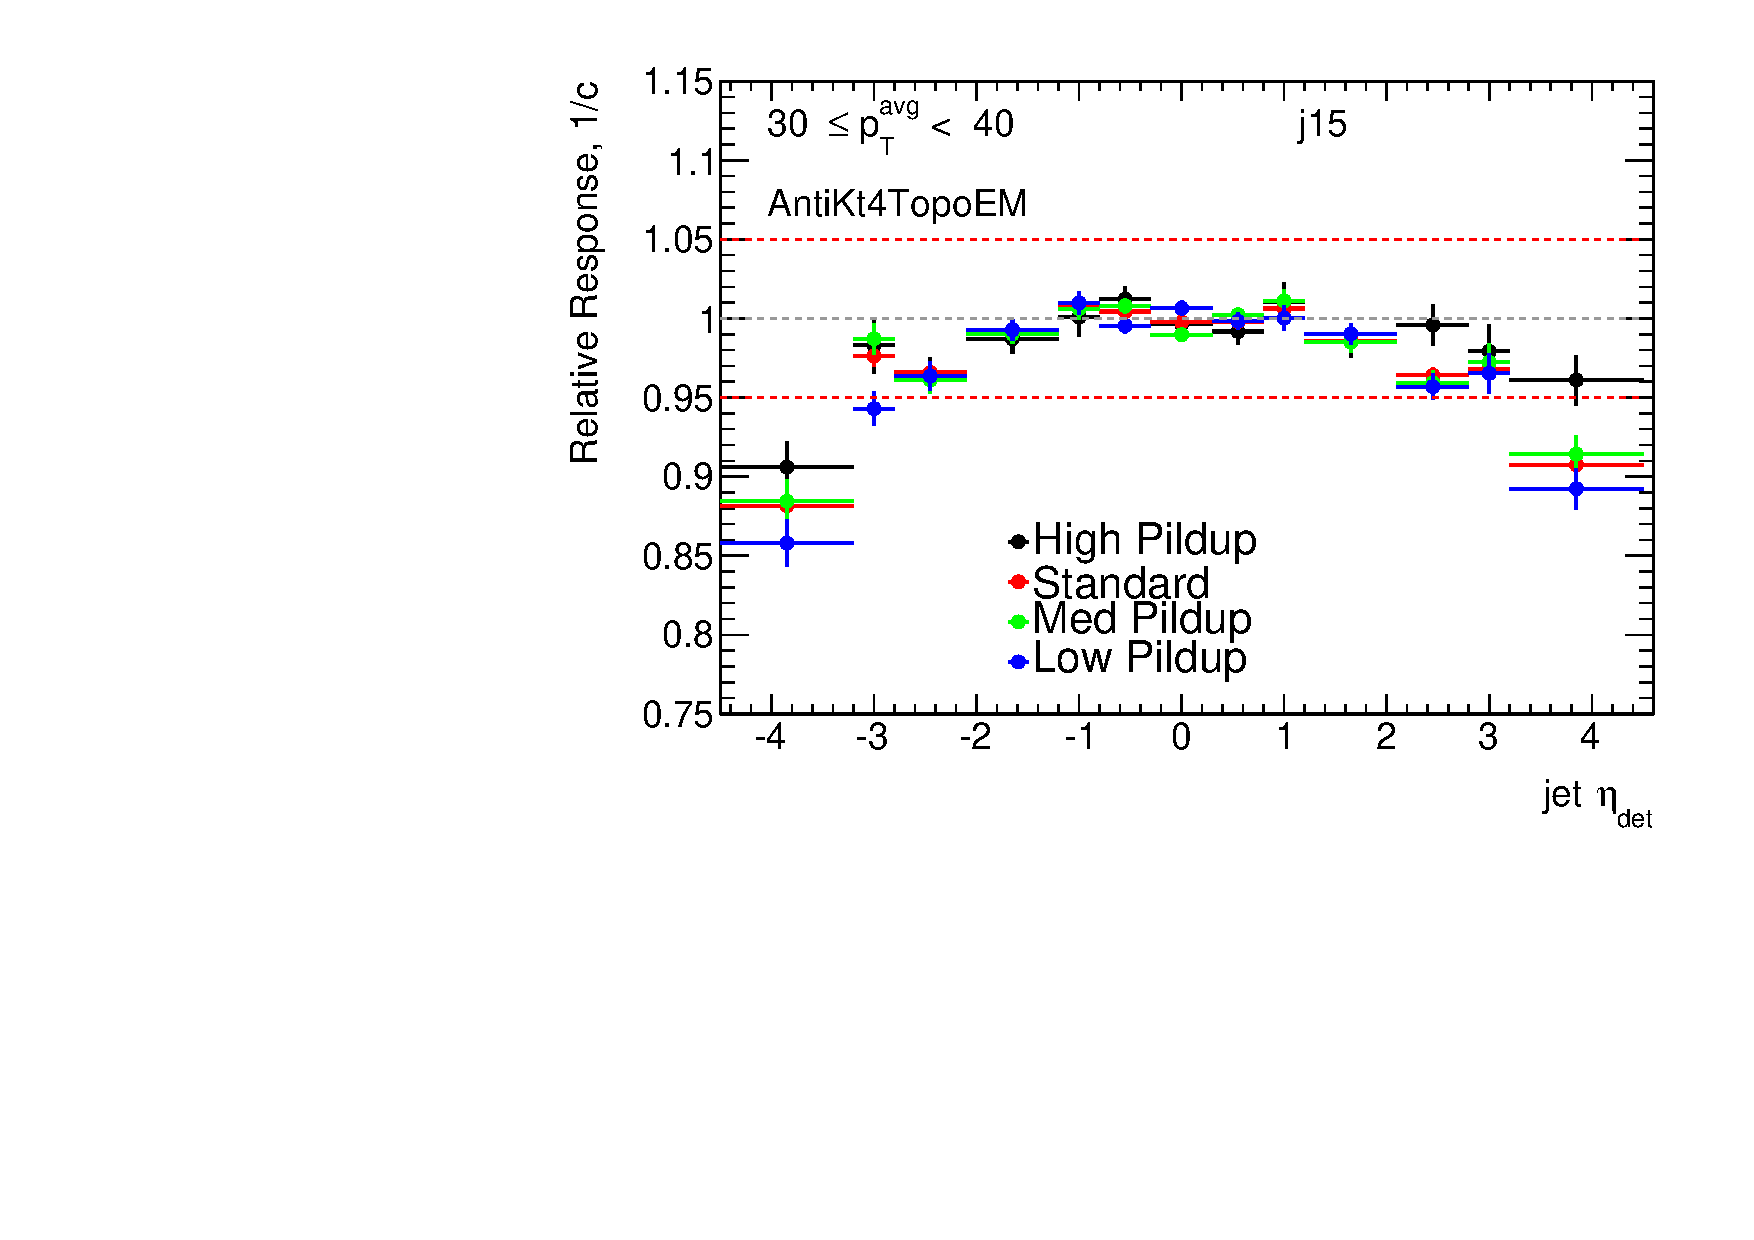
\includegraphics[width=0.8\textwidth]{figures/JetPerformance/2011/Pileup/PileupComp_AntiKt4TopoEM_j15_30-40Uncorrected.pdf}
}
\caption[]{
Relative response as a function of detector $\eta$ for jets with $30<\ptave{}<40$ GeV.
Relative responses are shown for events with \Range{NPV}{0}{2}, \Range{NPV}{3}{6}, $\rm NPV\ge7$ and all NPV. 
\label{JetPerf:PileupComp_j15}}
\end{figure}

\begin{figure}
\centering
\mbox{
              \epsfig{figure=figures/JetPerformance/2011/ResponseNPVj30Comp.eps,width=0.9\textwidth}
              %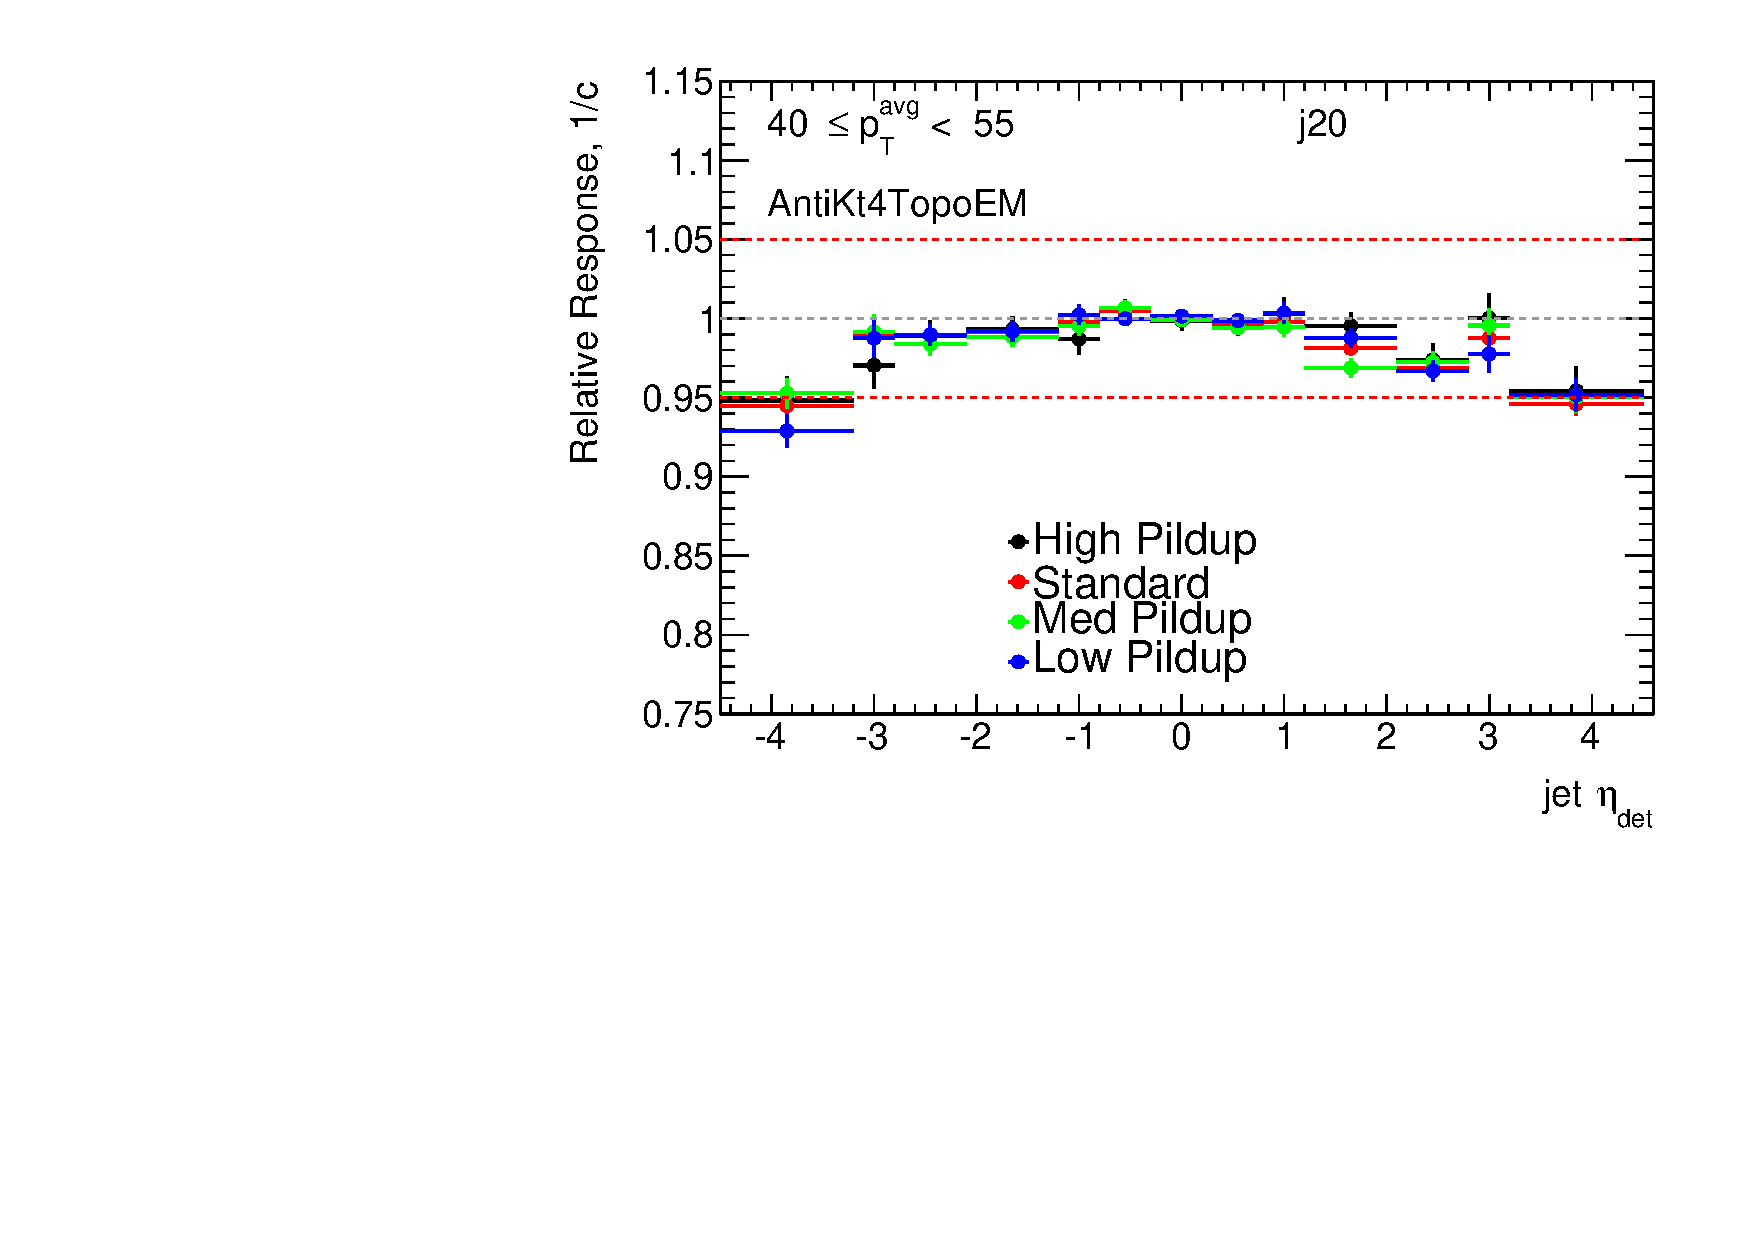
\includegraphics[width=0.8\textwidth]{figures/JetPerformance/2011/Pileup/PileupComp_AntiKt4TopoEM_j20_40-55Uncorrected.pdf}
}
\caption[]{
Relative response as a function of detector $\eta$ for jets with $55<\ptave{}<75$ GeV.
Relative responses are shown for events with \Range{NPV}{0}{2}, \Range{NPV}{3}{6}, $\rm NPV\ge7$ and all NPV. 
\label{JetPerf:PileupComp_j20}}
\end{figure}

\begin{figure}
\centering
\mbox{
              \epsfig{figure=figures/JetPerformance/2011/Responsemuj10Comp.eps,width=0.9\textwidth}
              %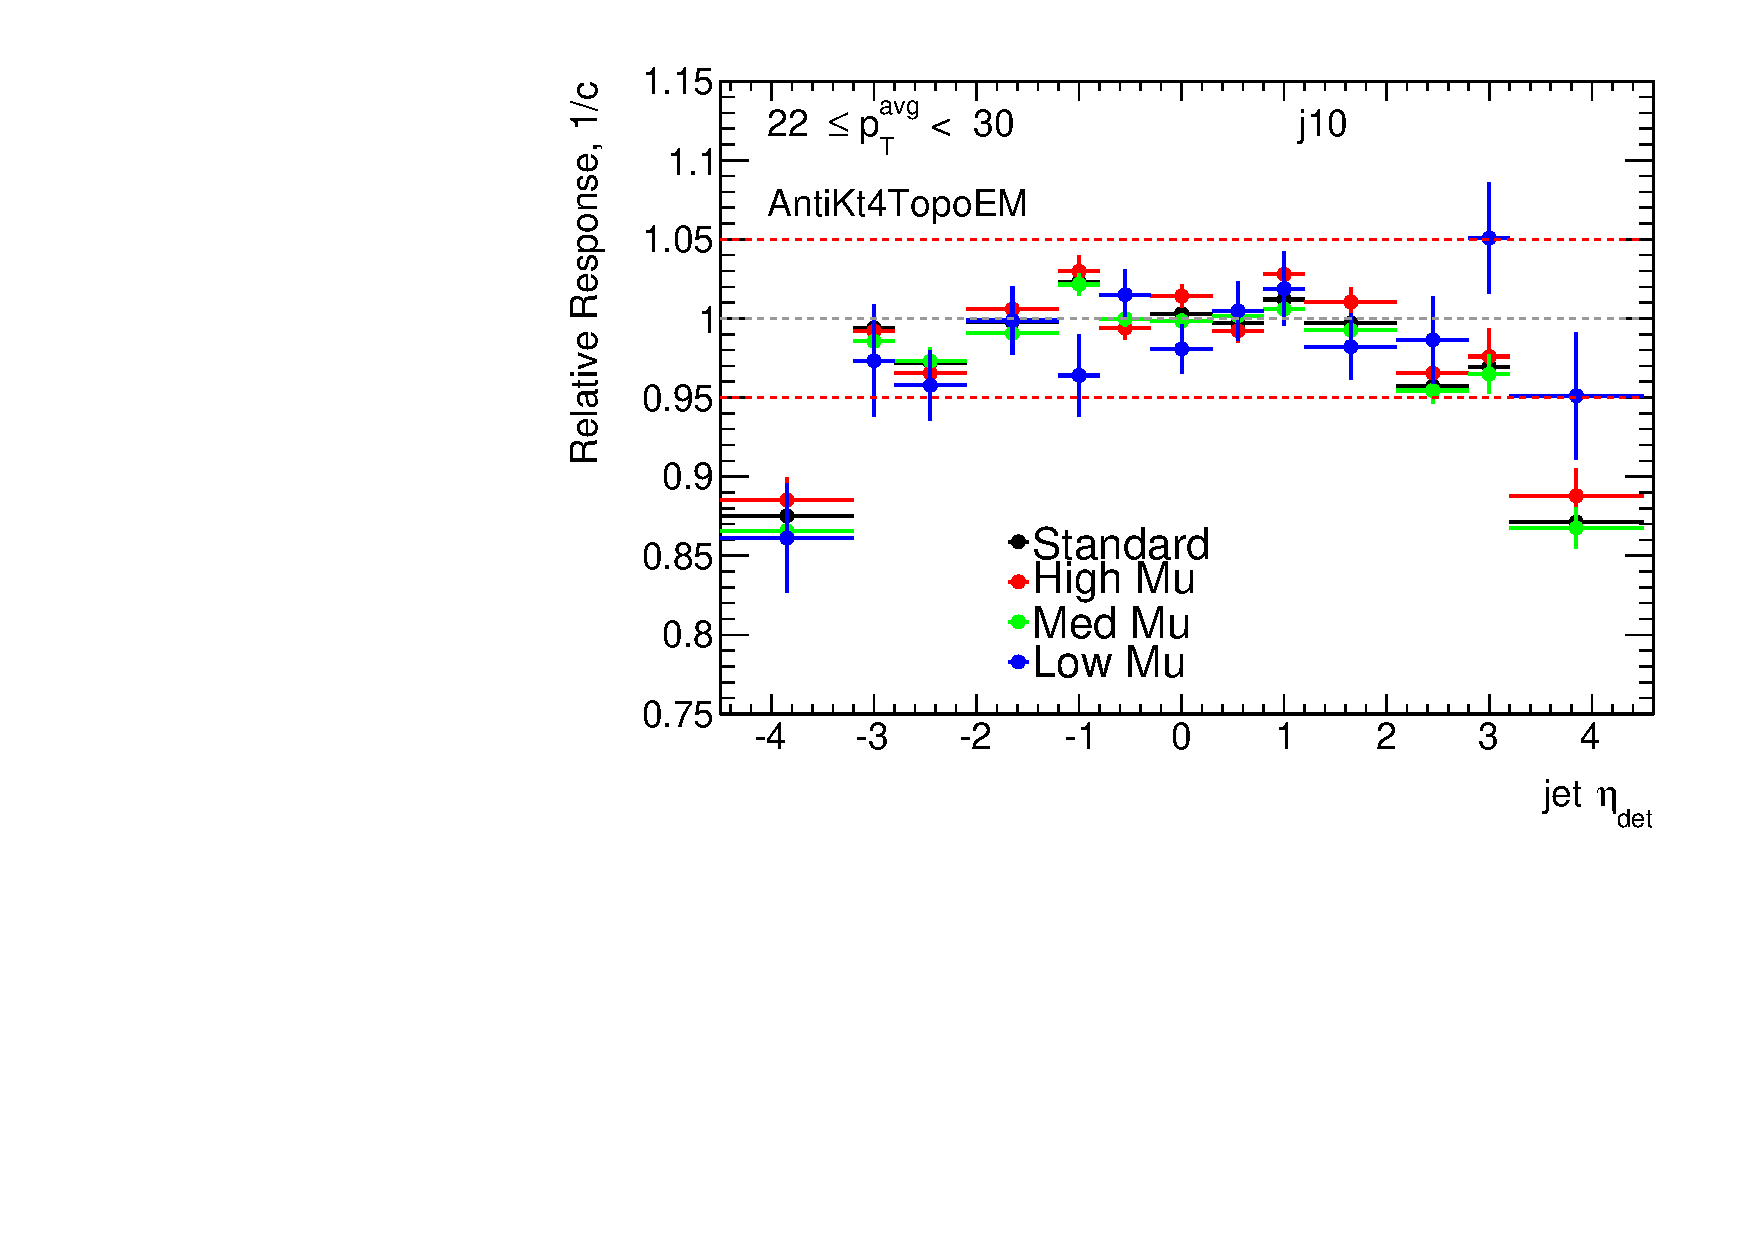
\includegraphics[width=0.8\textwidth]{figures/JetPerformance/2011/Pileup/MuComp_AntiKt4TopoEM_j10_22-30Uncorrected.pdf}
}
\caption[]{
Relative response as a function of detector $\eta$ for jets with $22<\ptave{}<30$ GeV.
Relative responses are shown for events with \Range{\mu}{0}{6}, $\rm \mu\ge6$ and all $\mu$. 
\label{JetPerf:MuComp_j10}}
\end{figure}



\begin{figure}
\centering
\mbox{
              \epsfig{figure=figures/JetPerformance/2011/Responsemuj15Comp.eps,width=0.9\textwidth}
              %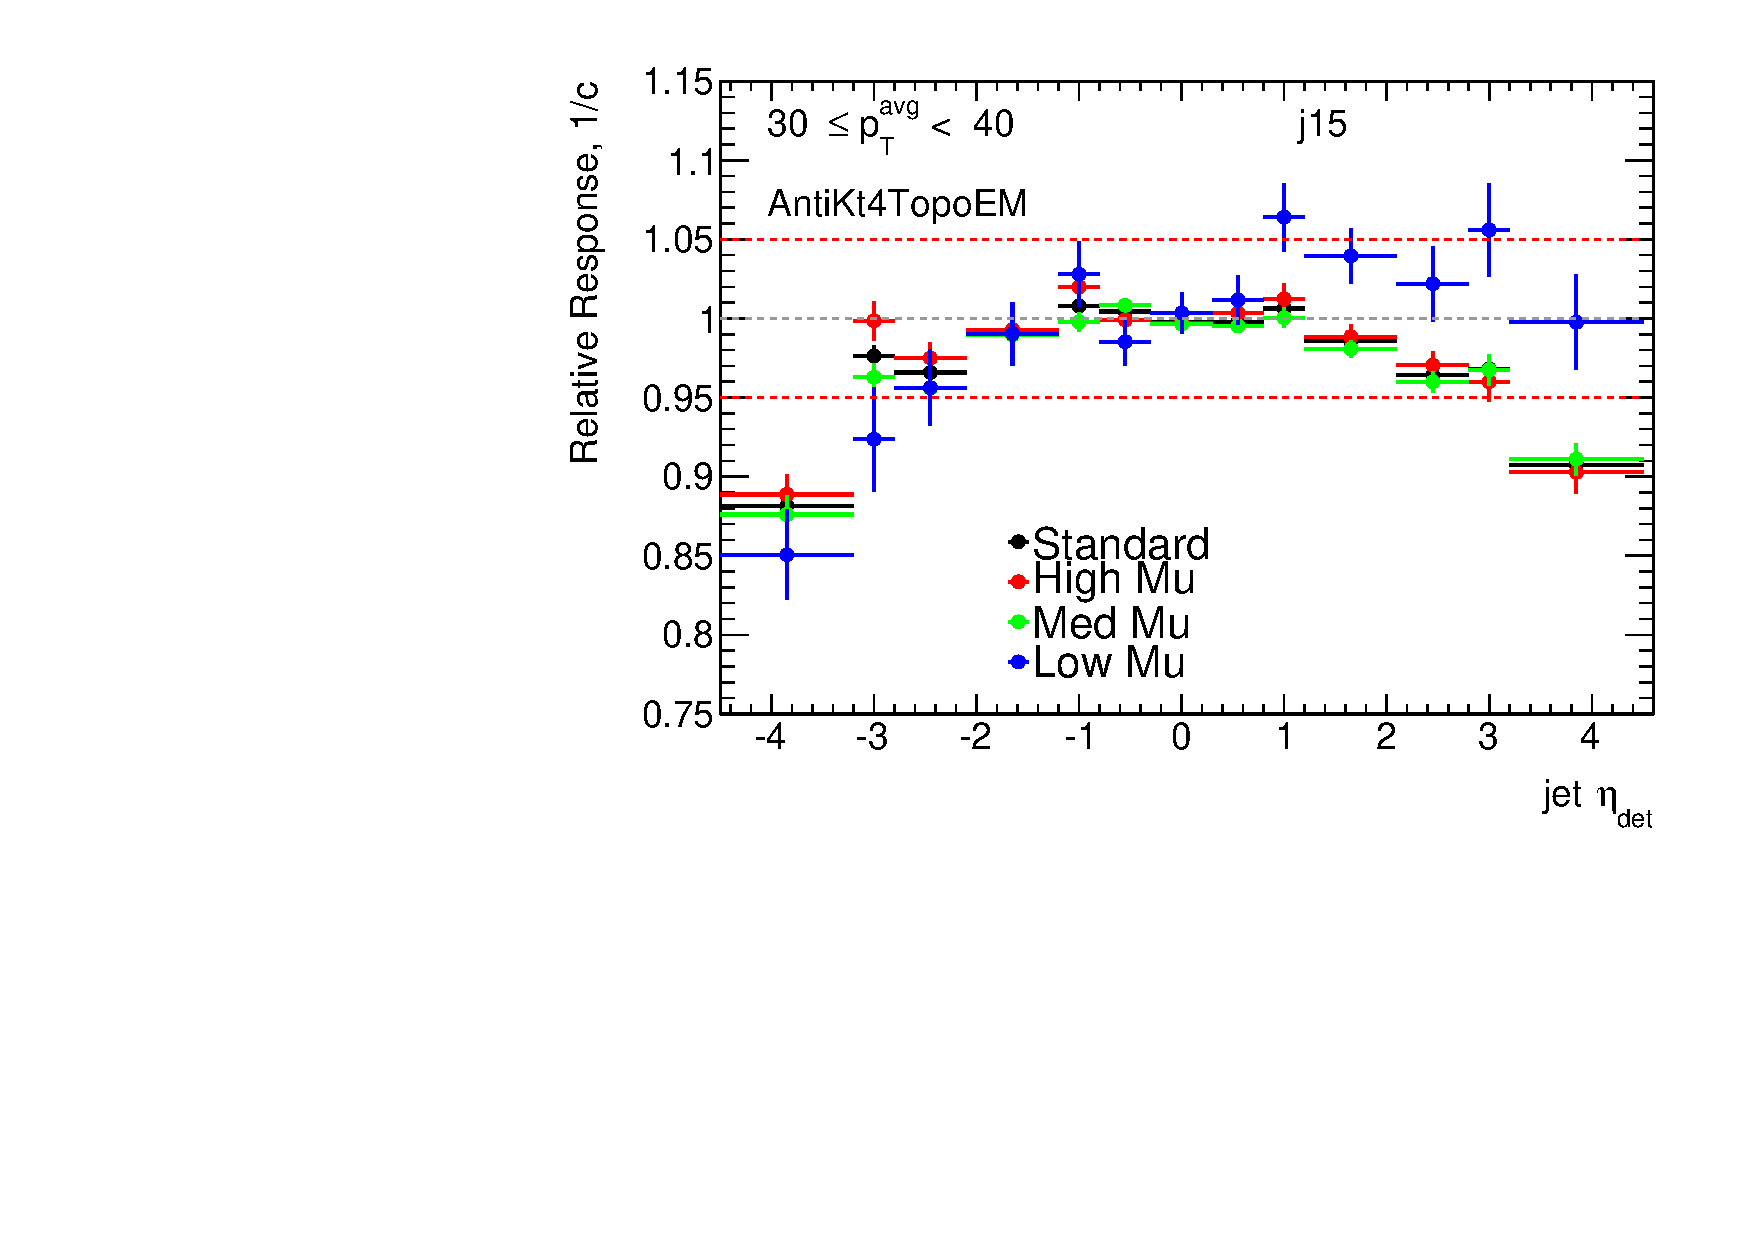
\includegraphics[width=0.8\textwidth]{figures/JetPerformance/2011/Pileup/MuComp_AntiKt4TopoEM_j15_30-40Uncorrected.pdf}
}
\caption[]{
Relative response as a function of detector $\eta$ for jets with $30<\ptave{}<40$ GeV.
Relative responses are shown for events with \Range{\mu}{0}{6}, $\rm \mu\ge6$ and all $\mu$. 
\label{JetPerf:MuComp_j15}}
\end{figure}

\begin{figure}
\centering
\mbox{
              \epsfig{figure=figures/JetPerformance/2011/Responsemuj30Comp.eps,width=0.9\textwidth}
              %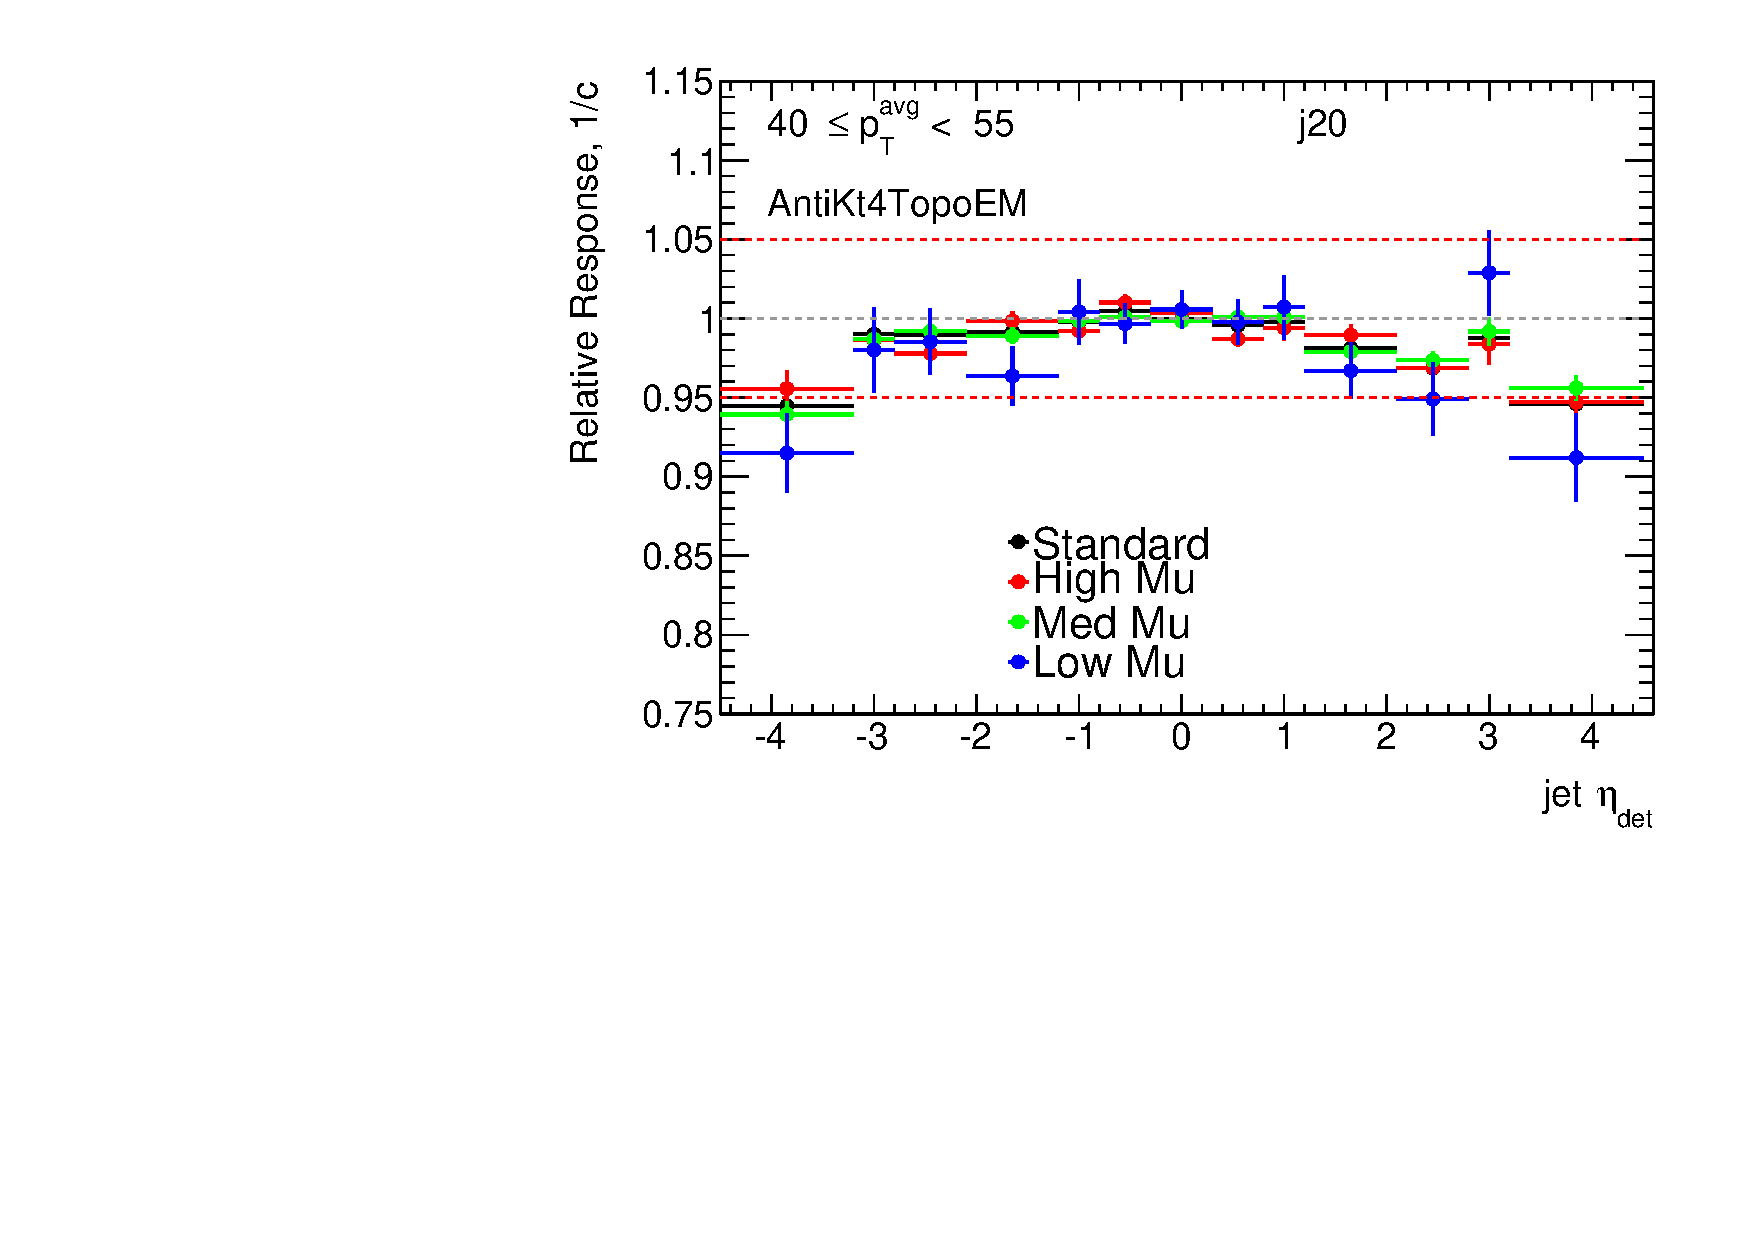
\includegraphics[width=0.8\textwidth]{figures/JetPerformance/2011/Pileup/MuComp_AntiKt4TopoEM_j20_40-55Uncorrected.pdf}
}
\caption[]{
Relative response as a function of detector $\eta$ for jets with $55<\ptave{}<75$ GeV.
Relative responses are shown for events with \Range{\mu}{0}{6}, $\rm \mu\ge6$ and all $\mu$. 
\label{JetPerf:MuComp_j20}}
\end{figure}

